\documentclass[10pt,a4paper]{article}
\usepackage[utf8]{inputenc}
\usepackage[a4paper,%
            left=.75in,right=.75in,top=1in,bottom=1in]{geometry}
\setlength{\headsep}{0.25in}

\usepackage{amsthm}

\usepackage{graphicx}
\usepackage{pgfplots}
            
\usepackage[english]{babel}

\theoremstyle{theorem}
\newtheorem{theorem}{Theorem}
\newtheorem{lemma}{Lemma}
\newtheorem{corollary}{Corollary}
\newtheorem{case}{Case}

\usepackage{amsthm}
\usepackage{lipsum}
\usepackage{tikz}

\makeatletter
\newcommand{\proofpart}[2]{%
  \par
  \addvspace{\medskipamount}%
  \noindent\emph{Part #1: #2}\par\nobreak
  \addvspace{\smallskipamount}%
  \@afterheading
}
\makeatother

\newcommand\restr[2]{{% we make the whole thing an ordinary symbol
  \left.\kern-\nulldelimiterspace % automatically resize the bar with \right
  #1 % the function
  \vphantom{\big|} % pretend it's a little taller at normal size
  \right|_{#2} % this is the delimiter
  }}

\theoremstyle{definition}
\newtheorem{definition}{Definition}
\newtheorem{remark}{Remark}

\usepackage{mathtools}
\DeclarePairedDelimiter\bra{\langle}{\rvert}
\DeclarePairedDelimiter\ket{\lvert}{\rangle}
\DeclarePairedDelimiterX\braket[2]{\langle}{\rangle}{#1 \delimsize\vert #2}

\usepackage{amsmath}
\usepackage{amsfonts}
\usepackage{amssymb}
\usepackage{fancyhdr}
\usepackage{tkz-euclide}

\DeclareMathOperator{\interior}{int}

\newcommand{\Tau}{\mathcal{T}}

\newenvironment{amatrix}[1]{%
  \left(\begin{array}{@{}*{#1}{c}|c@{}}
}{%
  \end{array}\right)
}

\usepackage{calligra}
\DeclareMathAlphabet{\mathcalligra}{T1}{calligra}{m}{n}
\DeclareFontShape{T1}{calligra}{m}{n}{<->s*[2.2]callig15}{}

\newcommand{\scripty}[1]{\ensuremath{\mathcalligra{#1}}}

\pagestyle{fancy}
\author{Jeremiah Givens}
\newcommand{\subject}{Real Analysis II}
\newcommand{\Date}{9/2/2021} 
\makeatletter
\rhead{{\small\@author}}
\lhead{{\small\subject}}
\chead{{\large Homework 1}}
\cfoot{}
\rfoot{\thepage}
\lfoot{\today}

\renewcommand{\theequation}{\arabic{equation}}

\begin{document}
\section*{Problem 1}
Let 
\[   f = \left\{
\begin{array}{ll}
      \frac{xy}{(x^2 + y^2)^2} & \text{if } (x, y) \in [-1, 1]^2 \backslash \{(0, 0)\} \\
      0 & \text{if } (x, y) = (0, 0)\\
\end{array} 
\right. \]

Show that 
\begin{align*}
\int_{-1}^1 \left( \int_{-1}^1 f(x, y) dy \right) dx = \int_{-1}^1 \left( \int_{-1}^1 f(x, y) dx \right) dy,
\end{align*}
but $f \not \in L([-1, 1]^2)$.

\subsection*{Solution}
We have, for any $x \in [-1, 1]$,
\begin{align*}
\int_{-1}^1 f(x, y) dy &= \int_{-1}^1 \frac{xy}{(x^2 + y^2)^2} dy\\
&= 0 &&\text{Since we are integrating and odd function over symmetric bounds}
\end{align*}
With an identical argument, we have that for any $y \in [0, 1]$,
\begin{align*}
\int_{-1}^1 f(x, y) dy &= \int_{-1}^1 \frac{xy}{(x^2 + y^2)^2} dy\\
&= 0.
\end{align*}
Thus,
\begin{align*}
0 = \int_{-1}^1 \left( \int_{-1}^1 f(x, y) dy \right) dx = \int_{-1}^1 \left( \int_{-1}^1 f(x, y) dx \right) dy.
\end{align*}

Now, to show that $f \not \in L([-1, 1]^2)$, we will show that $|f| \not \in L([-1, 1]^2)$. We have
\[   |f| = \left\{
\begin{array}{ll}
      \frac{|x||y|}{(x^2 + y^2)^2} & \text{if } (x, y) \in [-1, 1]^2 \backslash \{(0, 0)\} \\
      0 & \text{if } (x, y) = (0, 0)\\
\end{array} 
\right. \]
Since this $|f|$ is continuous almost everywhere, we have that $|f|$ is measurable. Thus, by Tonneli's theorem, we have
\begin{align*}
\int \int_{[-1, 1]^2} |f(x, y)| dy dx &= \int_{-1}^1 \left( \int_{-1}^1 |f(x, y)| dy \right) dx\\
&= \int_{-1}^1 \left( 2\int_{0}^1 |f(x, y)| dy \right) dx &&\text{Even function over symmetric bounds}\\
&= \int_{-1}^1 \left( 2\int_{0}^1 \frac{|x|y}{(x^2 + y^2)^2} dy \right) dx\\
&= \int_{-1}^1 \left( \int_{u(0)}^{u(1)} |x| u^{-2} du \right) dx && \text{u sub with } u = x^2 + y^2\\
&= \int_{-1}^1 \left. \left( -|x| u^{-1} \right) \right|_{u(0)}^{u(1)} dx\\
&= \int_{-1}^1 \left. \left( -\frac{|x|}{x^2 + y^2} \right) \right|_{0}^{1} dx\\
&= \int_{-1}^1 \left( \frac{|x|}{x^2} -\frac{|x|}{x^2 + 1} \right) dx\\
&= 2\int_{0}^1 \left( \frac{x}{x^2} -\frac{x}{x^2 + 1} \right) dx&&\text{Even function over symmetric bounds}\\
\end{align*}
\begin{align*}
&= 2\int_{0}^1 \left( \frac{1}{x} -\frac{x}{x^2 + 1} \right) dx\\
&= \infty - \int_{1}^2 u^{-1} du &&\text{u sub with } u = x^2 + 1\\
&= \infty - \ln (2)\\
&= \infty.
\end{align*}
Thus, we have shown that $f \not \in L([-1, 1]^2)$.

\section*{Problem 2}
\begin{theorem}
Let $A \subseteq \mathbb{R}^p$ be measurable, and $B \subseteq \mathbb{R}^q$ be non-measurable with $|B|_e < \infty$. Then
\proofpart{(i)}{} If $|A| = 0$, then $A \times B$ is measurable, and
\proofpart{(ii)}{} If $|A| > 0$, then $A \times B$ is not measurable.
\end{theorem}

\subsection*{Solution}
\begin{proof}
\proofpart{(i)}{} Suppose $|A|=0$. Define $H \subseteq \mathbb{R}^q$ such that $H \subseteq B$, $H$ is of type $G_\delta$, and $|H| = |B|_e$. Then, we have
\begin{align*}
|A \times B|_e &\leq |A \times H| &&\text{Since } A \times B \subseteq A \times H\\
&= |A| \cdot |H|\\
&= |A| \cdot |B|_e\\
&= 0 \cdot |B|_e\\
&= 0 && \text{Since } |B|_e < \infty.
\end{align*}
Thus, $A \times B$ is measurable.
\end{proof}

\proofpart{(ii)}{} We will prove the contrapositive. Thus, suppose $A \times B$ is measurable. Then, by the first theorem we proved in class this semester, we have that for almost every $x \in \mathbb{R}^p$, $(A \times B)_x$ is measurable. Now, by definition, we have that for $x \in A$, 
\begin{align*}
(A \times B)_x = B,
\end{align*} 
and for $x \not \in A$, 
\begin{align*}
(A \times B)_x = \emptyset.
\end{align*}
Thus, for almost every $x \in A$, we have that $B$ is measurable. However, since we know $B$ is not measurable, we can conclude that $A$ is a set of measure zero, and our proof of the contrapostive is complete.

\section*{Problem 3}
Show that
\begin{align*}
\int \int_{[0, \infty]^2} \frac{dx dy}{(1 + x)(1 + x y^2)} = \frac{\pi^2}{2}.
\end{align*}

\subsection*{Solution}
Since our integrand is continuous, it is measurable. Thus, since we also have that our integrand is nonnegative, Tonneli's theorem allows us to compute this as an itterated integral:
\begin{align*}
\int \int_{[0, \infty]^2} \frac{dx dy}{(1 + x)(1 + x y^2)} &= \int_0^\infty \frac{1}{(1 + x)} \left( \int_0^\infty \frac{1}{1 + x y^2} dy \right) dx\\
&= \int_0^\infty \frac{1}{x(1 + x)} \left( \int_0^\infty \frac{1}{\frac{1}{x} + y^2} dy \right) dx\\
&= \int_0^\infty \frac{1}{x(1 + x)} \left( \frac{\pi \sqrt{x}}{2} \right) dx &&\text{Integral table}\\
&= \frac{\pi}{2}\int_0^\infty \frac{1}{\sqrt{x}(1 + x)} dx\\
&= \frac{\pi^2}{2} &&\text{Integral table}.
\end{align*}

\section*{Problem 4}
Let $f(x, y) = e^{-y} \sin(2xy)$ for $(x, y) \in E = [0, 1] \times [0, \infty)$. Apply Fubini's theorem to show
\begin{align*}
\int_0^\infty e^{-y} \frac{sin^2 y}{y} dy = \frac{1}{4} \ln 5.
\end{align*}

\subsection*{Solution}
Since $f$ is continuous, $f$ is measurable, and the classical formula presented at the beginning of chapter 6 tells us that the integral of $f$ will be equal to it's iterated integral.

Now, we note that for $y \in [0, \infty)$, we have
\begin{align*}
\int_0^1 e^{-y} \sin(2xy) dx = e^{-y} \frac{sin^2 y}{y}.
\end{align*}
Thus, using Fubini's theorem, we have
\begin{align*}
\int_0^\infty e^{-y} \frac{sin^2 y}{y} dy &= \int_0^\infty \left( \int_0^1 e^{-y} \sin(2xy) dx \right) dy\\
&= \int_0^1 \left(\int_0^\infty e^{-y} \sin(2xy) dy \right) dx\\
&= \int_0^1 \frac{2x}{4x^2 + 1} dx && \text{After two applications of integration by parts}\\
&= \int_{u(0)}^{u(1)} \frac{du}{4u} && \text{u sub with } u = 4x^2 + 1\\
&= \left. \frac{1}{4}\ln(4x^2 + 1) \right|_0^1\\
&= \frac{1}{4} \ln 5.
\end{align*}
If you would like to see the work for integration by parts, let me know, and I can send you a picture of my white board.

\section*{Problem 5}
\begin{theorem}
\proofpart{(i)}{} Let $f$ be measurable on $\mathbb{R}^p$, and $g$ be measurable on $\mathbb{R}^q$. Then $h(x, y) = f(x)g(x)$ is measurable on $\mathbb{R}^{p + q}$.

\proofpart{(ii)}{} Let $f \in L(\mathbb{R}^p)$, and $g \in L(\mathbb{R}^q)$. Then $h(x, y) = f(x)g(y) \in L(\mathbb{R}^{p + q})$ and 
\begin{align*}
\int \int_{\mathbb{R}^{p + q}} f(x)g(y) dx dy = \left(\int_{\mathbb{R}^{p}} f(x) dx\right) \left( \int_{\mathbb{R}^{q}} g(y) dy \right).
\end{align*}
\end{theorem}

\begin{proof}
\proofpart{(i)}{} Define $\bar{f}(x, y) = f(x)$ and $\bar{g}(x, y) = g(y)$ for all $(x, y) \in \mathbb{R}^{p + q}$. Then, for any $a \in \mathbb{R}$, we have
\begin{align*}
\{\bar{f} > a \} = \{f > a \} \times \mathbb{R}^q \text{, and } \{\bar{g} > a \} = \mathbb{R}^p \times \{g > a \}.
\end{align*}
Now, since $f$ and $g$ are measurable, and (as we proved last semester) the cartesian product of measurable sets is measurable, we can conclude that $\bar{f}$ and $\bar{g}$ are measurable. Finally, since $h = \bar{f} \cdot \bar{g}$, theorem 4.10 in our textbook tells us that $h$ is measurable.

\proofpart{(ii)}{} Define $h(x, y)$ as we did in part (i). By theorem 4.6, we have that $|h(x, y)| = |f(x)| \cdot |g(y)|$ is measurable. Thus, by Tonneli's theorem, we have
\begin{align*}
\int \int_{\mathbb{R}^{p + q}} |h(x, y)| dx dy &= \int_{\mathbb{R}^{p}} \left( \int_{\mathbb{R}^{q}} |h(x, y)| dy \right) dx\\
&= \int_{\mathbb{R}^{p}} \left( \int_{\mathbb{R}^{q}} |f(x)||g(y)| dy \right) dx\\
&= \left(\int_{\mathbb{R}^{p}} |f(x)| dx\right) \left( \int_{\mathbb{R}^{q}} |g(y)| dy \right) && \text{Since there is no } x \text{ dependence in } \int_{\mathbb{R}^{q}} |g(y)| dy.
\end{align*}
Thus, since $f$ and $g$ are integrable, the two integrals in the last expression are finite, and we can conclude that $h$ is integrable. Finally, since $h$ is integrable, Fubini's theorem tells us
\begin{align*}
\int \int_{\mathbb{R}^{p + q}} f(x)g(y) dx dy &= \int_{\mathbb{R}^{p}} \left( \int_{\mathbb{R}^{q}} f(x)g(y) dy \right) dx\\
&= \left(\int_{\mathbb{R}^{p}} f(x) dx\right) \left( \int_{\mathbb{R}^{q}} g(y) dy \right)&& \text{Since there is no } x \text{ dependence in } \int_{\mathbb{R}^{q}} g(y) dy.
\end{align*}
With this, our proof is complete.
\end{proof}

\section*{Problem 6}
Let $f(x, y) = \frac{x^2 - y^2}{x^2 + y^2}$ for $(x, y) \not = (0, 0)$. Show that 
\begin{align*}
\int_0^1 \left(\int_0^1 f(x, y)dy \right) dx = 0. 
\end{align*}

\subsection*{Solution}
First, let us examine the inner most integral
\begin{align*}
\int_0^1 \frac{x^2 - y^2}{x^2 + y^2}dy.
\end{align*}
As we normally do for integrals of this form, we will draw a triangle, and use this to make some handy variable changes.
\begin{center}
\begin{tikzpicture}
\coordinate (A) at (0, 0);
\coordinate (B) at (4, 0);
\coordinate (C) at (4, 4);
	\draw (A) -- (B) node[midway, below]{$x$} -- (C) node[midway, right]{$y$} -- cycle node[midway, left]{$\sqrt{x^2 + y^2}$};
	\tkzMarkAngle[size=1cm,color=cyan, mark=](B,A,C)
	\tkzLabelAngle[pos=1.2](B,A,C){$\theta$}
\end{tikzpicture}
\end{center}
Thus, using this, we let 
\begin{align*}
y &= x\tan\theta\\
dy &= x \sec^2 \theta d \theta\\
\cos \theta &= \frac{x}{\sqrt{x^2 + y^2}},
\end{align*}
With this change of variables, our integral becomes
\begin{align*}
\int_0^1 \frac{x^2 - y^2}{x^2 + y^2}dy &= \int_{\theta(0)}^{\theta(1)} x(2 - \sec^2 \theta)dy\\
&= \left. (2x \theta - x\tan \theta ) \right|_{\theta(0)}^{\theta(1)}\\
&= \left. \left(2x \tan^{-1}\left(\frac{y}{x}\right) - x\frac{y}{x} \right) \right|_0^1\\
&= 2x \tan^{-1}\left(\frac{1}{x}\right) - 1.
\end{align*}
Now, we can solve the final integral:
\begin{align*}
\int_0^1 \left(\int_0^1 f(x, y)dy \right) dx &= \int_0^1 \left(2x \tan^{-1}\left(\frac{1}{x}\right) - 1 \right) dx\\
&= -1 + \int_0^1 2x \tan^{-1}\left(\frac{1}{x}\right) dx\\
\end{align*}
Once again, we will draw a triangle to help determine an appropriate change of variables:
\begin{center}
\begin{tikzpicture}
\coordinate (A) at (0, 0);
\coordinate (B) at (4, 0);
\coordinate (C) at (4, 4);
	\draw (A) -- (B) node[midway, below]{$x$} -- (C) node[midway, right]{$1$} -- cycle node[midway, left]{$\sqrt{x^2 + 1}$};
	\tkzMarkAngle[size=1cm,color=cyan, mark=](B,A,C)
	\tkzLabelAngle[pos=1.2](B,A,C){$\theta$}
\end{tikzpicture}
\end{center}
With this, we have
\begin{align*}
\tan^{-1} \left(\frac{1}{x} \right) &= \theta\\
\sin^{-2} \theta &= x^2 + 1\\
x &= \cot \theta\\
dx &= - (\csc \theta)^2
\end{align*}
Thus, plugging these subsitutions in and making some simplifications, we have
\begin{align*}
-1 + \int_0^1 2x \tan^{-1}\left(\frac{1}{x}\right) dx &= -1 - 2 \int_{\theta(0)}^{\theta(1)} \theta \frac{\cos \theta}{\sin^3 \theta} d \theta.
\end{align*}
Now, recognizing that 
\begin{align*}
\frac{d}{d \theta} \left( \theta (\sin \theta)^{-2} \right) &= csc^2(\theta) - 2 \theta \frac{\cos \theta}{\sin^3 \theta}
\end{align*}
we can use integration by parts to reduce our integral to
\begin{align*}
-1 - 2 \int_{\theta(0)}^{\theta(1)} \theta \frac{\cos \theta}{\sin^3 \theta} d \theta &= -1 + \left. \theta \sin^{-2} \theta \right|_{\theta(0)}^{\theta(1)} - \int_{\theta(0)}^{\theta(1)} \csc^2 \theta d \theta \\
&= -1 + \left. \theta \sin^{-2} \theta \right|_{\theta(0)}^{\theta(1)} + \left. \cot \theta \right|_{\theta(0)}^{\theta(1)}\\
&= -1 + \left. (x^2 + 1) \tan^{-1} \left(\frac{1}{x} \right) \right|_0^1 +  \left. x \right|_0^1\\
&= -1 + 2\frac{\pi}{4} - \frac{\pi}{2} + 1\\
&= 0,
\end{align*}
as desired.

\section{Problem 7}
\begin{theorem}
\proofpart{(a)}{} Let $E$ be a measurable subset of $\mathbb{R}^2$ such that for almost every $x \in \mathbb{R}^1$, $\{y : (x, y) \in E \}$ has measure zero. Then $E$ has measure 0, and for almost every $y \in \mathbb{R}^1$, $\{x : (x, y) \in E \}$ has measure zero. 
\proofpart{(b)}{} Let $f(x, y)$ be nonnegative and measurable in $\mathbb{R}^2$. Suppose that for almost every $x \in \mathbb{R}$, $f(x, y)$ is finite for almost every $y$. Then, for almost every $y \in \mathbb{R}$, $f(x, y)$ is finite for almost every $x$.
\end{theorem}

\subsection*{Solution}
\begin{proof}
\proofpart{(a)}{} Define $A,B \subseteq \mathbb{R}$ such that $E = A \times B$. We have that for $x \in A$, 
\begin{align*}
\{y : (x, y) \in E \} = B,
\end{align*}
and for $x \not \in A$,
\begin{align*}
\{y : (x, y) \in E \} = \emptyset.
\end{align*}
Thus, either $|B| = 0$, or $|A| = 0$. Armed with this information, let's examine the set $\{x : (x, y) \in E \}$. We have that for $y \in B$,
\begin{align*}
\{x : (x, y) \in E \} = A,
\end{align*}
and for $y \not \in B$,
\begin{align*}
\{x : (x, y) \in E \} = \emptyset.
\end{align*}
If $|A| = 0$, it follows that this set has zero measure for all $y$. Suppose now that $|B| = 0$. Then, for almost every $y$ (that is, the ones not in the measure zero set $B$), we have that $\{x : (x, y) \in E \} = \emptyset$, which implies it has measure zero.

Now, we must show that $E$ has measure zero. Suppose first that $|A| = 0$. Let $H \subseteq \mathbb{R}$ be of type $G_\delta$ with $B \subseteq H$, and $|H| = |B|_e$. Then, we have
\begin{align*}
|A \times B|_e &\leq |A \times H| &&\text{Since } A \times B \subseteq A \times H\\
&= |A| \cdot |H| &&\text{We proved this in class for measurable sets}\\
&= 0 \cdot |H|\\
&= 0.
\end{align*}
Thus, $|E| = 0$. The case of $|B| = 0$ can be handled in a nearly identical fashion.

\proofpart{(b)}{} Since for almost every $x \in \mathbb{R}$, $f(x, y)$ is finite for almost every $y$, there exist zero measure sets $A, B \subseteq \mathbb{R}$ such that for every $x \in \mathbb{R} \backslash A$, and for every $y \in \mathbb{R} \backslash B$, $f(x, y)$ is finite. Thus, for every $y \in \mathbb{R} \backslash B$, $f(x, y)$ is finite for every $x \in \mathbb{R} \backslash A$. Thus, by direct definition of "almost everywhere", we have that for almost every $y \in \mathbb{R}$, $f(x, y)$ is finite for almost every $x$.
\end{proof}

\section*{Problem 8}
If $f$ and $g$ are measurable in $\mathbb{R}^n$ show that $h(x, y) = f(x)g(y)$ is measurable in $\mathbb{R}^n \times \mathbb{R}^n$. Deduce that if $E_1$ and $E_2$ are measurable subsets of $\mathbb{R}^n$, then their cartesian product is measurable.

\subsection*{Solution}
We proved the first part of this in part (i) of problem 5. We proved the second part of this problem in class last semester at the start of chapter 5 (you proved a more general version of Lemma 5.2 in the book).

\section*{Problem 9}
\begin{theorem}
Let $f$ be measurable on $(0, 1)$. If $f(x) - f(y)$ is integrable over the square $[0, 1]^2$, show that $f \in L(0, 1)$.
\end{theorem}

\subsection*{Solution}
\begin{proof}
Since $f(x) - f(y)$ is integrable over the square $[0, 1]^2$, Fubini's theorem tells us
\begin{align*}
\int \int_{[0, 1]^2} (f(x) - f(y)) dx dy &= \int_0^1 \left( \int_0^1 (f(x) - f(y)) dy \right) dx\\
&= \int_0^1 \left(f(x) - \int_0^1 f(y) dy \right) dx &&f(x) \text{ acts as a constant when integrating over }y\\
&= \int_0^1 f(x) dx - \int_0^1 f(y) dy &&\int_0^1 f(y) \text{ acts as a constant when integrating over }x.
\end{align*}
Thus, since $f(x) - f(y)$ is integrable over the square $[0, 1]^2$, the integral must be finite. From this, we can conclude that the last two integrals on the write side must me finite, and we have shown that $f \in L(0, 1)$.
\end{proof}

\section*{Problem 10}
\begin{theorem}
Let $A \subseteq \mathbb{R}^p$ be measurable, and let $B \subseteq \mathbb{R}^q$ be an arbitrary set. Then
\begin{align*}
|A \times B|_e = |A| \cdot |B|_e.
\end{align*}
\end{theorem}

\subsection*{Solution}
\begin{proof}
Let $H \subseteq \mathbb{R}^q$ be of type $G_\delta$ such that $B \subseteq H$ and $|B|_e = |H|$. Then,
\begin{align*}
|A \times B|_e &\leq |A \times H| &&\text{Since } A \times B \subseteq A \times H\\
&= |A| \cdot |H|\\
&= |A| \cdot |B|_e.
\end{align*}
Now, to show inequality in the reverse direction, let $U \subseteq \mathbb{R}^{p + q}$ be of type $G_\delta$ such that $|U| = |A \times B|_e$. We have
\begin{align*}
|A \times B|_e &= |U|\\
&= \int \int_U \chi_U dx dy\\
&= \int_{\mathbb{R}^p} \left( \int_{U_x} \chi_U dy \right) dx &&\text{By Fubini's theorem}\\
&\geq \int_{A} \left( \int_{U_x} \chi_U dy \right) dx &&\text{Since } A \subseteq \mathbb{R}^p\\
&= \int_A |U_x| dx\\
&\geq \int_A |B|_e &&\text{Since } B \subseteq U_x\\
&= |A| \cdot |B|_e.
\end{align*}
Thus, we have shown that $|A \times B|_e = |A| \cdot |B|_e$, and our proof is complete.
\end{proof}

\end{document}